\documentclass[11pt,a4paper]{article}
\usepackage[T1]{fontenc}
\usepackage[utf8]{inputenc}
\usepackage{lmodern}
\usepackage[margin=1in]{geometry}
\usepackage{amsmath,amssymb,amsthm,mathtools}
\usepackage{booktabs,microtype,graphicx,array}
\usepackage[colorlinks=true,linkcolor=blue,citecolor=blue,urlcolor=blue]{hyperref}
\newtheorem{theorem}{Theorem}[section]
\newtheorem{proposition}[theorem]{Proposition}
\newtheorem{lemma}[theorem]{Lemma}
\newtheorem{corollary}[theorem]{Corollary}
\newtheorem{conjecture}[theorem]{Conjecture}
\theoremstyle{definition}
\newtheorem{definition}[theorem]{Definition}
\theoremstyle{remark}
\newtheorem{remark}[theorem]{Remark}
\newcommand{\dd}{\,\mathrm{d}}
\newcommand{\Disc}{\operatorname{Disc}}
\newcommand{\Nzero}{\mathbb{N}_0}
\newcommand{\bc}{b_{\mathrm c}}
\newcommand{\LP}{\mathcal{L\!-\!P}}
\title{Nonreal poles of Weniger's delta transformation\\ for Stieltjes series}
\author{Anonymous}
\date{23 October 2026\\[2pt]\small Version 1.0.0-candidate (unrefereed). DOI: \href{https://doi.org/10.5281/zenodo.23586255}{10.5281/zenodo.23586255}.\\
\small Code and data: \url{https://github.com/ipitchford/weniger-delta-nonreal-poles}}

\begin{document}
\maketitle

\begin{abstract}
The standard (diagonal and near-diagonal) Padé approximants to a Stieltjes
series have their poles on the negative real axis, where the function has its branch cut. Borghi (2026)
asked whether Weniger's delta transformation, a faster alternative for
divergent series, shares this property. We show that in general it does
not, and we say exactly when it does. For every Stieltjes measure the
denominator has only negative real zeros at orders one and two; at order
three this holds exactly when $n+\beta\le(\sqrt{33}-5)/2$, where $n$ is the
starting index and $\beta$ the shift; from order four on, no choice of
$n$ and $\beta$ protects every measure. The reason is simple: positive
moments can be tuned so that only three consecutive coefficients of the
denominator matter, and from order four the delta weights fail the
classical factor-four test for those three. The nonreal zeros are genuine
poles. For one fixed measure we prove that nonreal denominator zeros occur
at every sufficiently large order, and we certify genuine nonreal poles
exactly at every order from 3 to 30. On the positive side, real-rootedness
holds at every order whenever the reciprocal moments form a multiplier
sequence, or the moment ratios $\mu_{r+1}/\mu_r$ increase at least
fourfold at each step. Borghi proved real-rootedness for the
superfactorial, Laguerre and integer-difference Jacobi families at his
normalisation (starting index $0$, shift $1$); one proof extends these
cases to every starting index, shift and order. Exact rational-arithmetic
certificates accompany every finite claim.
\end{abstract}

\noindent\textbf{Keywords:} Stieltjes series; Weniger delta transformation;
Levin-type transformations; real zeros; multiplier sequences; Padé
approximation.\\
\textbf{MSC 2020:} 65B10, 41A21, 30C15, 26C10, 44A60.

\section{Introduction}\label{sec:intro}

\paragraph{Why pole location matters.}
A Stieltjes function $f(z)=\int_0^\infty(z+t)^{-1}\dd\mu(t)$ is analytic
off the cut $(-\infty,0]$, and its asymptotic series at infinity often
diverges. Padé approximants are the classical tool for summing such
series. Their convergence theory rests on one structural fact: the
denominators are orthogonal polynomials for $\mu$, so every pole is simple,
lies on the cut and carries a positive residue \cite[Ch.~5]{BakerGM1996}.
Levin-type transformations \cite{Levin1973,Weniger1989,Sidi2003,
BrezinskiRZ1991,Homeier2000}, and in particular Weniger's delta
transformation \cite{Weniger1989}, are often much faster than Padé on
factorially divergent Stieltjes series \cite{BorghiWeniger2015}; for
some hypergeometric data Levin-type approximants even coincide with Padé
approximants \cite{Sidi1981}, and Slevinsky derives stable recurrences for
the Drummond and factorial Levin-type rational approximants to generalised
hypergeometric functions, with results on the placement of their poles
\cite{Slevinsky2025}. Whether
they also place their poles on the cut is therefore the natural first
question for any convergence theory of them.

\paragraph{The question.}
Borghi \cite[\S3.1]{Borghi2026} poses it as follows. Writing his
equation~(23) for the delta transformation, he asks:
\begin{quote}
``Is it true that all zeros of the denominator of Equation (23) are
confined to the sole negative real axis?''
\end{quote}
In \S3.3 he specialises: ``Henceforth, for the sake of simplicity but
without loss of generality, it will be assumed'' that the starting index is
$0$ and the shift is $1$. He then writes the denominator $Q_k$ as a
$(k-1)$-fold derivative of $z^{k-1}P_k(z)$, where
$P_k(z)=\sum_j\binom kj z^j/\mu_{n+1+j}$ (our \eqref{eq:borghiP}), and uses
the Gauss--Lucas theorem to argue that differentiation pulls the zeros
towards the axis. He states that ``only two scenarios are possible: (i)
all zeros or (ii) not all zeros of'' $P_k$ ``are real'', that in scenario
(i) all zeros of $Q_k$ are real and negative, and that in scenario (ii)
``the problem of proving the reality of zeros of'' $Q_k$ ``remains open''.
He describes the full claim as ``a well-grounded conjecture'' and notes
that a proof that the convex hull collapses onto the axis ``for any
Stieltjes sequence'' is open \cite[\S3.3]{Borghi2026}. His measure class is
the one used here: a positive measure on $[0,\infty)$ with infinitely many
points of increase and all moments finite. Our $\beta$ is the parameter
$\gamma$ in the published article's equations (23) and (26); the author
preprint uses $\beta$ in its equations (26) and (29).

\paragraph{The answer.}
The conjecture is false, already at $n=0$, $\beta=1$ and order three. All
our counterexamples lie in Borghi's scenario (ii), the case his argument
leaves open (Remark~\ref{rem:scenario}). More precisely, call the pair
$(k;n,\beta)$ \emph{universally safe} if $Q_k^{(n,\beta)}$ has only negative
real zeros for every admissible measure. Table~\ref{tab:classification}
gives the complete answer.

\begin{table}[htbp]
\centering
\caption{Universal safety of the delta denominator, by order $k$ and shift
$b=n+\beta$ (Theorem~\ref{thm:main}). ``Unsafe'' means some admissible
measure gives a genuine nonreal conjugate pair of poles.}
\label{tab:classification}
\begin{tabular}{@{}p{0.12\linewidth}p{0.42\linewidth}p{0.38\linewidth}@{}}
\toprule
Order $k$ & Universally safe & Unsafe\\
\midrule
$1,2$ & every $n\ge0$, $\beta>0$ & never\\
$3$ & exactly $b\le\bc=(\sqrt{33}-5)/2\approx0.3723$ (so $n=0$, $\beta\le\bc$) & $b>\bc$; e.g.\ every $n\ge1$, and $\beta=1$\\
$\ge4$ & never & every $n\ge0$, $\beta>0$\\
\bottomrule
\end{tabular}
\end{table}

\paragraph{The mechanism in one paragraph.}
The denominator is $Q_k(z)=\sum_j h_j z^j/\mu_{m+j}$ with fixed weights
$h_j=\binom kj(b+j)_{k-1}$ and $m=n+1$. The explicit measures below make three consecutive normalised moments
approach equality in log-convexity while the neighbouring moments diverge,
so the moments are huge at every index of the window except three
consecutive ones; then $Q_k$ is, up to a negligible error, $z^{j-1}$ times the quadratic
$h_{j-1}+h_jz+h_{j+1}z^2$. Such a quadratic has nonreal roots exactly when
$h_j^2<4h_{j-1}h_{j+1}$. Conversely, if every ratio
$h_j^2/(h_{j-1}h_{j+1})$ is at least $4$, the classical
Hutchinson--Kurtz criterion forces real zeros for every measure. For the
delta weights the top ratio is below $10/3$ as soon as $k\ge4$, and it is
below $4$ at $k=3$ exactly when $b>\bc$.

\paragraph{Contributions.} Classical inputs are the factor-four criterion
\cite{Hutchinson1923,Kurtz1992}, Pólya--Schur multiplier sequences
\cite{PolyaSchur1914,CravenCsordas1989}, accuracy-through-order
\cite{Homeier2000} and Hankel positivity. New here are:
\begin{enumerate}
\item the complete order--shift classification (Theorem~\ref{thm:main}),
via a realisation lemma: any three consecutive reciprocal-moment
coefficients can be isolated by positive measures
(Theorem~\ref{thm:universalcoefficients});
\item proofs that the nonreal zeros are genuine poles; for every fixed $n$,
one measure defeating every shift at order four, and an explicit such
measure for $n=0$ and $n=1$ (\S\ref{sec:examples});
\item a persistence theorem: $Q_k(w/k^2)$ converges to an entire function
$E_\mu$, so nonreal zeros of $E_\mu$ force nonreal denominator zeros at
all large orders; for one fixed measure this gives nonreal zeros at all
large orders, and exact certificates give genuine nonreal poles at every
order $3\le k\le30$ (\S\ref{sec:persistence});
\item a positive theorem (\S\ref{sec:positive}). Borghi proved
real-rootedness at starting index $0$ and shift $1$ for the integer
superfactorial and Laguerre moments and for Jacobi weights whose
parameters differ by an integer \cite[\S\S4.2, 4.3, 4.6]{Borghi2026}; one
operator proof extends these cases to every $n$, $\beta$ and $k$, and
to $\Gamma(\nu\ell+c)$ for every $c>0$. We add practical guidance with an
exact diagnostic (\S\ref{sec:practice}).
\end{enumerate}
Table~\ref{tab:status} lists every result with its exact status.

\begin{table}[htbp]
\centering
\caption{Status of the results. ``Proof'' means a complete mathematical
proof in the text; ``certificate'' means an exact rational computation in
\texttt{code/verify\_all.py}; ``numerical'' means floating point,
illustrative only.}
\label{tab:status}
\small
\begin{tabular}{@{}p{0.52\linewidth}p{0.40\linewidth}@{}}
\toprule
Result & Status\\
\midrule
Classification, Table~\ref{tab:classification} (Thm~\ref{thm:main}) & proof\\
Genuine poles in the classification & proof\\
Explicit examples, $k=3,4$; tail family $k=5$--$8$ (Table~\ref{tab:tail}) & certificate\\
One measure, all shifts, $k=4$, $n\in\{0,1\}$ (Prop.~\ref{prop:allshift}) & certificate of a polynomial identity in $\beta$\\
One measure, all shifts, $k=4$, every fixed $n$ (Cor.~\ref{cor:allshifts}) & proof\\
Limit $Q_k(w/k^2)\to E_\mu$ (Thm~\ref{thm:limit}) & proof\\
Fixed measure: nonreal zeros at all large $k$ (Thm~\ref{thm:persist}) & proof plus one exact certificate\\
Fixed measure: genuine nonreal poles, $3\le k\le30$ & certificate\\
Fixed measure: genuine nonreal poles at every $k\ge3$ (Conj.~\ref{conj:persist}) & open\\
Positive criteria (Thm~\ref{thm:positive}, Cor.~\ref{cor:families}) & proof\\
Natural families real-rooted on a grid, $\beta\le5$ (\S\ref{sec:positive}) & certificate\\
All shifts real-rooted iff $P_k$ is (Rem.~\ref{rem:largeshift}) & proof\\
Pole locations, residues, accuracy (\S\ref{sec:practice}) & numerical\\
\bottomrule
\end{tabular}
\end{table}

\paragraph{Roadmap.}
Section~\ref{sec:setting} fixes notation and treats orders one and two.
Section~\ref{sec:criterion} proves the reciprocal-moment criterion.
Section~\ref{sec:classification} proves the classification, including
genuineness of the poles; the cubic discriminant computation is in
Appendix~\ref{app:cubic}. Section~\ref{sec:examples} gives explicit
examples. Sections~\ref{sec:persistence}--\ref{sec:practice} contain the
persistence theorem, the positive theorem and the practical discussion.
Section~\ref{sec:scope} states the limits of the results and open
problems. Appendix~\ref{app:repro} describes the certificates.

\section{Setting and low orders}\label{sec:setting}

Let $\mu$ be a positive Borel measure on $[0,\infty)$ with infinite support
and finite moments
\begin{equation}\label{eq:moments}
 \mu_\ell=\int_0^\infty t^\ell\dd\mu(t),\qquad \ell\in\Nzero .
\end{equation}
We call such $\mu$ \emph{admissible}. Then
$f(z)=\int_0^\infty(z+t)^{-1}\dd\mu(t)\sim\sum_{\ell\ge0}(-1)^\ell\mu_\ell
z^{-\ell-1}$, with partial sums
$f_n(z)=\sum_{\ell=0}^n(-1)^\ell\mu_\ell z^{-\ell-1}$. For $k\ge1$,
$n\in\Nzero$ and $\beta>0$ the delta transformation is
\cite{Weniger1989}, \cite[eq.~(23)]{Borghi2026}
\begin{equation}\label{eq:delta}
 \delta_k^{(n)}(\beta;z)
 =\frac{\Delta^k\{(n+\beta)_{k-1}f_n(z)/\Delta f_n(z)\}}
        {\Delta^k\{(n+\beta)_{k-1}/\Delta f_n(z)\}},
\end{equation}
where $\Delta$ acts on $n$ and $(a)_r=a(a+1)\cdots(a+r-1)$. Throughout,
\[
 b=n+\beta>0,\qquad m=n+1 .
\]
Since $\Delta f_{n+j}(z)=(-1)^{n+j+1}\mu_{n+j+1}z^{-n-j-2}$,
\begin{equation}\label{eq:DeltaQ}
 \Delta^k\Bigl\{\frac{(n+\beta)_{k-1}}{\Delta f_n(z)}\Bigr\}
 =(-1)^{n+k+1}z^{n+2}Q_k^{(n,\beta)}(z),\qquad
 Q_k^{(n,\beta)}(z)=\sum_{j=0}^k\binom{k}{j}\frac{(b+j)_{k-1}}{\mu_{m+j}}z^j,
\end{equation}
which is Borghi's eq.~(26). The same calculation in the numerator gives
\begin{equation}\label{eq:rational}
 \delta_k^{(n)}(\beta;z)=\frac{\sum_{j=0}^k a_jz^jf_{n+j}(z)}{Q_k(z)}
 =\frac{P_{n,k}(z)}{z^{n+1}Q_k(z)},\qquad
 a_j=\binom kj\frac{(b+j)_{k-1}}{\mu_{m+j}},
\end{equation}
with $P_{n,k}(z)=\sum_ja_j\sum_{\ell=0}^{n+j}(-1)^\ell\mu_\ell z^{n+j-\ell}$, a
real polynomial of degree at most $n+k$. We write
\begin{equation}\label{eq:borghiP}
 P_k(z)=\sum_{j=0}^k\binom kj\frac{z^j}{\mu_{m+j}}
\end{equation}
for Borghi's auxiliary polynomial \cite[eq.~(27)]{Borghi2026}. A zero of
$Q_k$ is a \emph{genuine pole} if it is not a zero of $P_{n,k}$, that is,
if it is a pole of the reduced rational function.

Cauchy--Schwarz for $t^r\dd\mu$ gives strict log-convexity,
\begin{equation}\label{eq:logconvex}
 \mu_r\mu_{r+2}>\mu_{r+1}^2\qquad(r\ge0),
\end{equation}
strict because equality would force $t^r\dd\mu$ to live on one point. All
counterexample measures below have moments $\mu_\ell\sim c\,\ell!$, so they
satisfy Carleman's condition $\sum\mu_\ell^{-1/(2\ell)}=\infty$ and the
moment problem is determinate \cite{Schmudgen2017}:
the failures are not artefacts of indeterminacy.

\begin{proposition}\label{prop:low}
For every admissible measure, $Q_1$ has one negative zero and $Q_2$ has two
distinct negative zeros.
\end{proposition}
\begin{proof}
$Q_1=\mu_m^{-1}+z\mu_{m+1}^{-1}$. For $Q_2=b\mu_m^{-1}+2(b+1)\mu_{m+1}^{-1}z
+(b+2)\mu_{m+2}^{-1}z^2$, by \eqref{eq:logconvex}
$\Disc(Q_2)=4\bigl((b+1)^2\mu_{m+1}^{-2}-b(b+2)\mu_m^{-1}\mu_{m+2}^{-1}\bigr)
\ge4\mu_{m+1}^{-2}>0$. Positive coefficients exclude zeros in $[0,\infty)$.
\end{proof}

\section{A reciprocal-moment criterion}\label{sec:criterion}

\begin{lemma}[Strict factor-four criterion \cite{Hutchinson1923,Kurtz1992}]\label{lem:four}
If $c_0,\dots,c_k>0$ and $c_j^2>4c_{j-1}c_{j+1}$ for $1\le j\le k-1$, then
$\sum_jc_jz^j$ has $k$ distinct negative zeros.
\end{lemma}
\begin{proof}
We include the short proof. Put $r_j=c_{j-1}/c_j$, so $r_{j+1}>4r_j$, and
$x_j=\sqrt{r_jr_{j+1}}$, $1\le j\le k-1$. Divide the value at $z=-x_j$ by
$(-1)^jc_jx_j^j$. The term of index $i$ becomes $(-1)^{i-j}T_i$ with
$T_i=c_ix_j^{i-j}/c_j>0$ and $T_j=1$. For $i\ge j$,
$T_{i+1}/T_i=x_j/r_{i+1}\le x_j/r_{j+1}<1$; for $i\le j$,
$T_{i-1}/T_i=r_i/x_j\le r_j/x_j<1$. So both tails are alternating with
decreasing moduli, and each is at least $-T_{j\pm1}=-\sqrt{r_j/r_{j+1}}>-1/2$.
Hence the polynomial has sign $(-1)^j$ at $-x_j$. As
$0<x_1<\dots<x_{k-1}$, the polynomial is positive at $0$ and has sign
$(-1)^k$ near $-\infty$, these sign changes give $k$ distinct negative zeros.
\end{proof}

\begin{theorem}[Fixed weights, arbitrary Stieltjes moments]\label{thm:universalcoefficients}
Fix $m\in\Nzero$, $k\ge1$ and $h_0,\dots,h_k>0$. The following are equivalent.
\begin{enumerate}
\item For every admissible measure, $q_{\mu}(z)=\sum_{i=0}^kh_iz^i/\mu_{m+i}$
has only negative real zeros.
\item $h_j^2\ge4h_{j-1}h_{j+1}$ for every internal index $1\le j\le k-1$.
\end{enumerate}
The zeros in 1 are then distinct. If 2 fails, a counterexample can be
chosen with a positive exponential density component and moments
$\sim c\,\ell!$.
\end{theorem}
\begin{proof}
\emph{Sufficiency.} For $c_i=h_i/\mu_{m+i}$,
$c_j^2/(c_{j-1}c_{j+1})=\bigl(h_j^2/(h_{j-1}h_{j+1})\bigr)\cdot
\mu_{m+j-1}\mu_{m+j+1}/\mu_{m+j}^2>4$ by \eqref{eq:logconvex}; apply
Lemma~\ref{lem:four}.

\emph{Necessity.} Suppose $h_j^2<4h_{j-1}h_{j+1}$. Put $r_\pm=m+j\pm1$ and,
for $K\ge2$,
\begin{equation}\label{eq:triplemeasure}
 \begin{aligned}
 \dd\mu^{\mathrm{tri}}_K&=\dd\delta_1+K^{2r_--1}\dd\delta_{K^{-2}}
 +K^{-2r_+-1}\dd\delta_{K^2}+K^{-1}e^{-t}\dd t,\\
 \mu_\ell&=1+K^{2(r_--\ell)-1}+K^{2(\ell-r_+)-1}+K^{-1}\ell! .
 \end{aligned}
\end{equation}
As $K\to\infty$, $\mu_\ell\to1$ for $\ell\in\{r_-,r_-+1,r_+\}$ and
$\mu_\ell\to\infty$ for the other $\ell\in[m,m+k]$. Hence $q_\mu\to
z^{j-1}(h_{j-1}+h_jz+h_{j+1}z^2)$ coefficientwise, so uniformly on
compact sets. The quadratic has two simple nonreal zeros; by Rouché's
theorem on small disjoint disks off the real axis, $q_\mu$ has nonreal
zeros for large $K$. Each $\mu^{\mathrm{tri}}_K$ is admissible with
$\mu_\ell\sim K^{-1}\ell!$.
\end{proof}

\begin{remark}[What is classical]\label{rem:classical}
Sufficiency is the Hutchinson--Kurtz criterion
\cite{Hutchinson1923,Kurtz1992}; on the history and sharpness of the
constant $4$ see Kostov and Shapiro \cite{KostovShapiro2013}. Necessity is
a realisation statement: three consecutive normalised Stieltjes moments
can be made arbitrarily close to the boundary configuration of equal
normalised moments while the neighbours dominate. This is in the spirit of classical moment-space
geometry \cite{Schmudgen2017}; we do not claim it as a new principle,
only its use for the delta classification. The preserver theorem of
Passare, Rojas and Shapiro \cite{Passare2011} concerns a different class
(sign-independently real-rooted polynomials): $(1,8,16,8,1)$ satisfies the
inequalities of Theorem~\ref{thm:universalcoefficients}, but
$1+8z-16z^2+8z^3+z^4$ has nonreal zeros.
\end{remark}

\section{Proof of the classification}\label{sec:classification}

\begin{theorem}[Order--shift classification]\label{thm:main}
Let $\bc=(\sqrt{33}-5)/2$ and $b=n+\beta$.
\begin{enumerate}
\item If $b\le\bc$, then for every admissible measure $Q_3^{(n,\beta)}$ has
three distinct negative zeros. The same holds for any positive quadruple
$(\mu_m,\dots,\mu_{m+3})$ satisfying the two log-convexity inequalities.
\item If $b>\bc$, some admissible measure gives $\delta_3^{(n)}(\beta;\cdot)$ a
genuine nonreal conjugate pair of poles.
\item Orders one and two are always safe (Proposition~\ref{prop:low}).
\item For every $k\ge4$, $n\ge0$, $\beta>0$, some admissible measure gives
$\delta_k^{(n)}(\beta;\cdot)$ a genuine nonreal conjugate pair of poles.
\end{enumerate}
In 2 and 4 the measure can be taken with a positive exponential density
component, moments $\sim c\,\ell!$, or (Corollary~\ref{cor:smooth}) with a
smooth positive density.
\end{theorem}

The proofs of parts 1--2 and 4 occupy \S\S\ref{sec:k4}--\ref{sec:genuine}.
The measure depends on $(k,n,\beta)$; \S\ref{sec:persistence} addresses one
fixed measure across orders.

\subsection{Orders four and above}\label{sec:k4}
For $h_j=\binom kj(b+j)_{k-1}$ the top internal ratio is
\begin{equation}\label{eq:tailratio}
 R_k(b)=\frac{h_{k-1}^2}{h_{k-2}h_k}
 =\frac{2k}{k-1}\frac{(b+k-1)(b+2k-3)}{(b+k-2)(b+2k-2)}
 =\frac{2k}{k-1}+\frac{2k}{(b+k-2)(b+2k-2)} .
\end{equation}
It decreases in $b>0$, so for $k\ge4$
\begin{equation}\label{eq:tailbound}
 R_k(b)<R_k(0)=\frac{k(2k-3)}{(k-1)(k-2)}\le\frac{10}{3}<4,
\end{equation}
the middle inequality being $(k-4)(4k-5)\ge0$. Theorem~\ref{thm:universalcoefficients}
gives nonreal zeros. For this top triple the right-hand atom of
\eqref{eq:triplemeasure} is not needed; the simpler family
\begin{equation}\label{eq:tailmeasure}
 \dd\mu^{\mathrm{tail}}_K=\dd\delta_1+K^{2\ell_0+1}\dd\delta_{K^{-2}}+K^{-1}e^{-t}\dd t,
 \qquad\ell_0=m+k-3,
\end{equation}
makes $Q_k$ converge to $z^{k-2}(h_{k-2}+h_{k-1}z+h_kz^2)$. Other internal
ratios often fail too (at $k=8$, $b\to0$, five of the seven are below
$4$), so the obstruction is robust.

\subsection{The cubic boundary}\label{sec:cubic}
At $k=3$ the two internal ratios are
$C^2/(BD)$ and $B^2/(CA)$ with $D=b(b+1)$, $C=3(b+1)(b+2)$,
$B=3(b+2)(b+3)$, $A=(b+3)(b+4)$, and
\[
 B^2-4AC=-3(b+2)(b+3)(b^2+5b-2),\qquad C^2-4BD=-3(b+1)(b+2)(b^2+3b-6).
\]
The first is nonnegative exactly for $b\le\bc$, the second for
$b\le\bc+1$. Hence Theorem~\ref{thm:universalcoefficients} gives part~1
(with distinct zeros) and the nonreal zeros in part~2. Appendix~\ref{app:cubic}
gives an independent discriminant proof of part~1 that also covers
non-strict log-convex quadruples, and an explicit family realising part~2.

\subsection{The nonreal zeros are genuine poles}\label{sec:genuine}

\begin{lemma}[Accuracy through order]\label{lem:accuracy}
For every admissible measure,
$\delta_k^{(n)}(\beta;z)-f(z)=O(z^{-n-k-3})$ as $z\to+\infty$. Consequently
the Laurent coefficients $r_\ell$ of the rational function
$\delta_k^{(n)}(\beta;z)=\sum_\ell r_\ell z^{-\ell-1}$ at infinity satisfy
$r_\ell=(-1)^\ell\mu_\ell$ for $0\le\ell\le n+k+1$.
\end{lemma}
\begin{proof}
This is the accuracy-through-order property of Levin-type transformations
\cite[\S6.3, Thm.~8]{Homeier2000}; we check it in the present convention.
For fixed $j$,
\[
 f_{n+j}(z)-f(z)=(-1)^{n+j}\mu_{n+j+1}z^{-n-j-2}+O(z^{-n-j-3})\qquad(z\to+\infty),
\]
by integrating the finite geometric remainder of $(z+t)^{-1}$.
In $\sum_ja_jz^j(f_{n+j}-f)$ the coefficient of $z^{-n-2}$ is
$(-1)^n\sum_j(-1)^j\binom kj(b+j)_{k-1}=0$, a $k$th difference of a
polynomial of degree $k-1$. Dividing by $Q_k$ (degree $k$, positive
leading coefficient) gives the bound. A rational function has a
convergent Laurent expansion at infinity, and an asymptotic expansion along
$z\to+\infty$ is unique; so the Laurent coefficients equal the asymptotic
ones.
\end{proof}

\begin{proposition}[Cancellation bound]\label{prop:noncancellation}
For every admissible measure,
$\deg\gcd(P_{n,k},Q_k^{(n,\beta)})<\lceil k/2\rceil$. In particular at
orders three and four no nonreal conjugate pair can cancel.
\end{proposition}
\begin{proof}
Suppose cancellation leaves a monic denominator factor $S(z)=\sum_{i=0}^r
s_iz^i$ with $r\le k/2$, so that $\delta=U/(z^mS)$ with $\deg U\le m+r-1$.
Since $S\delta=U/z^m$ has no terms below $z^{-m}$,
$\sum_is_ir_{m+i+j}=0$ for $0\le j\le r$. As $m+2r\le m+k$,
Lemma~\ref{lem:accuracy} turns this into
$(\mu_{m+i+j})_{i,j=0}^r(s_0,-s_1,\dots,(-1)^rs_r)^T=0$. This Hankel matrix
is positive definite, its quadratic form being
$\int t^m(\sum_iv_it^i)^2\dd\mu>0$ for $v\ne0$; contradiction with $s_r=1$.
A nonreal zero can only cancel together with its conjugate.
\end{proof}

For $k\ge5$ we exclude cancellation by moving one moment.

\begin{lemma}[Finitely many bad last moments]\label{lem:exceptional}
Fix $\mu_0,\dots,\mu_{n+k}>0$. As $\mu_{n+k+1}$ varies over $(0,\infty)$,
$P_{n,k}$ and $Q_k$ have a common zero for at most $k-1$ values.
\end{lemma}
\begin{proof}
Put $N=n+k$ and $Q_k=A+a_kz^k$, where only $a_k$ depends on $\mu_{N+1}$,
injectively. At a common zero $r\ne0$, eliminating $a_kr^k=-A(r)$ gives
$H(r)=0$ for $H(z)=z^{N+1}\sum_{j<k}a_jz^j(f_{n+j}(z)-f_N(z))$, a polynomial
with $\deg H\le k-1$ and $H(0)=-a_0(-1)^N\mu_N\ne0$. Each of its at most
$k-1$ zeros determines $a_k=-A(r)/r^k$.
\end{proof}

\begin{lemma}[Moving one moment inside the admissible class]\label{lem:momentperturbation}
Let $\mu$ contain $\varepsilon e^{-t}\dd t$, $\varepsilon>0$, and fix $L\ge1$.
With the shifted Legendre polynomial
$\psi_L(t)=\frac1{L!}\frac{\mathrm d^L}{\mathrm dt^L}[(t-1)^L(t-2)^L]$,
the measures $\mu+\theta\psi_L\mathbf 1_{[1,2]}\dd t$,
$|\theta|\,\|\psi_L\|_\infty<\varepsilon e^{-2}$, are admissible, have the
same moments of index $<L$, and have $L$th moment
$\mu_L+\theta(L!)^2/(2L+1)!$. Factorial asymptotics are preserved.
\end{lemma}
\begin{proof}
Integration by parts $L$ times gives $\int_1^2t^j\psi_L=0$ for $j<L$ and
$\int_1^2t^L\psi_L=(L!)^2/(2L+1)!$. The density stays positive, and the
change of the $\ell$th moment is $O(2^\ell)$.
\end{proof}

\begin{proof}[Proof of Theorem~\ref{thm:main}, parts 2 and 4]
Part~2: the construction of Appendix~\ref{app:cubic} and
Proposition~\ref{prop:noncancellation}. Part~4: the family
\eqref{eq:tailmeasure} gives a simple nonreal pair for large $K$; it
persists under small coefficient changes (Rouché). Apply
Lemma~\ref{lem:momentperturbation} with $L=n+k+1$ and choose the last moment
close to its old value and outside the finite set of
Lemma~\ref{lem:exceptional}. Then $P_{n,k}$ and $Q_k$ are coprime.
\end{proof}

\begin{corollary}[Smooth densities]\label{cor:smooth}
Every existence statement of Theorem~\ref{thm:main} holds with measures
having a $C^\infty$ strictly positive density on $(0,\infty)$ and moments
$\sim c\,\ell!$.
\end{corollary}
\begin{proof}
Take a coprime counterexample as above and convolve it with a $C^\infty$
probability density $\varphi$ on $\mathbb R$ supported in $[0,\eta]$ and
positive on $(0,\eta)$. The result has a $C^\infty$ density, positive on
$(0,\infty)$ (the exponential part already is); the indicator-cut Legendre
term becomes smooth after convolution. Finitely many moments move
continuously as $\eta\downarrow0$, and nonreal zeros in fixed disks and a
nonzero resultant are open conditions. Beyond a compact set the density
is a positive multiple of $e^{-t}$.
\end{proof}

\section{Explicit examples}\label{sec:examples}

All integers and identities in this section are recomputed by
\texttt{code/verify\_all.py} and listed in \texttt{results/verification.json};
we display only what a reader needs.

\paragraph{Order three, $n=0$, $\beta=1$.}
For $\dd\mu=\dd\delta_1+50\dd\delta_{1/50}+10^{-3}e^{-t}\dd t$,
$\mu_\ell=1+50^{1-\ell}+\ell!/1000$, the denominator is proportional to
\[
 \widehat Q(z)=1071932365000z^3+1963236457665z^2+966634623774z+54855937892,
\]
whose discriminant is a negative integer of $47$ digits. Exact Euclidean
division gives $\gcd(\widehat P,\widehat Q)=1$, with
$\delta_3^{(0)}(1;z)=\widehat P(z)/(1000z\widehat Q(z))$. The poles are
shown in Figure~\ref{fig:poles}.

\begin{figure}[htbp]
\centering
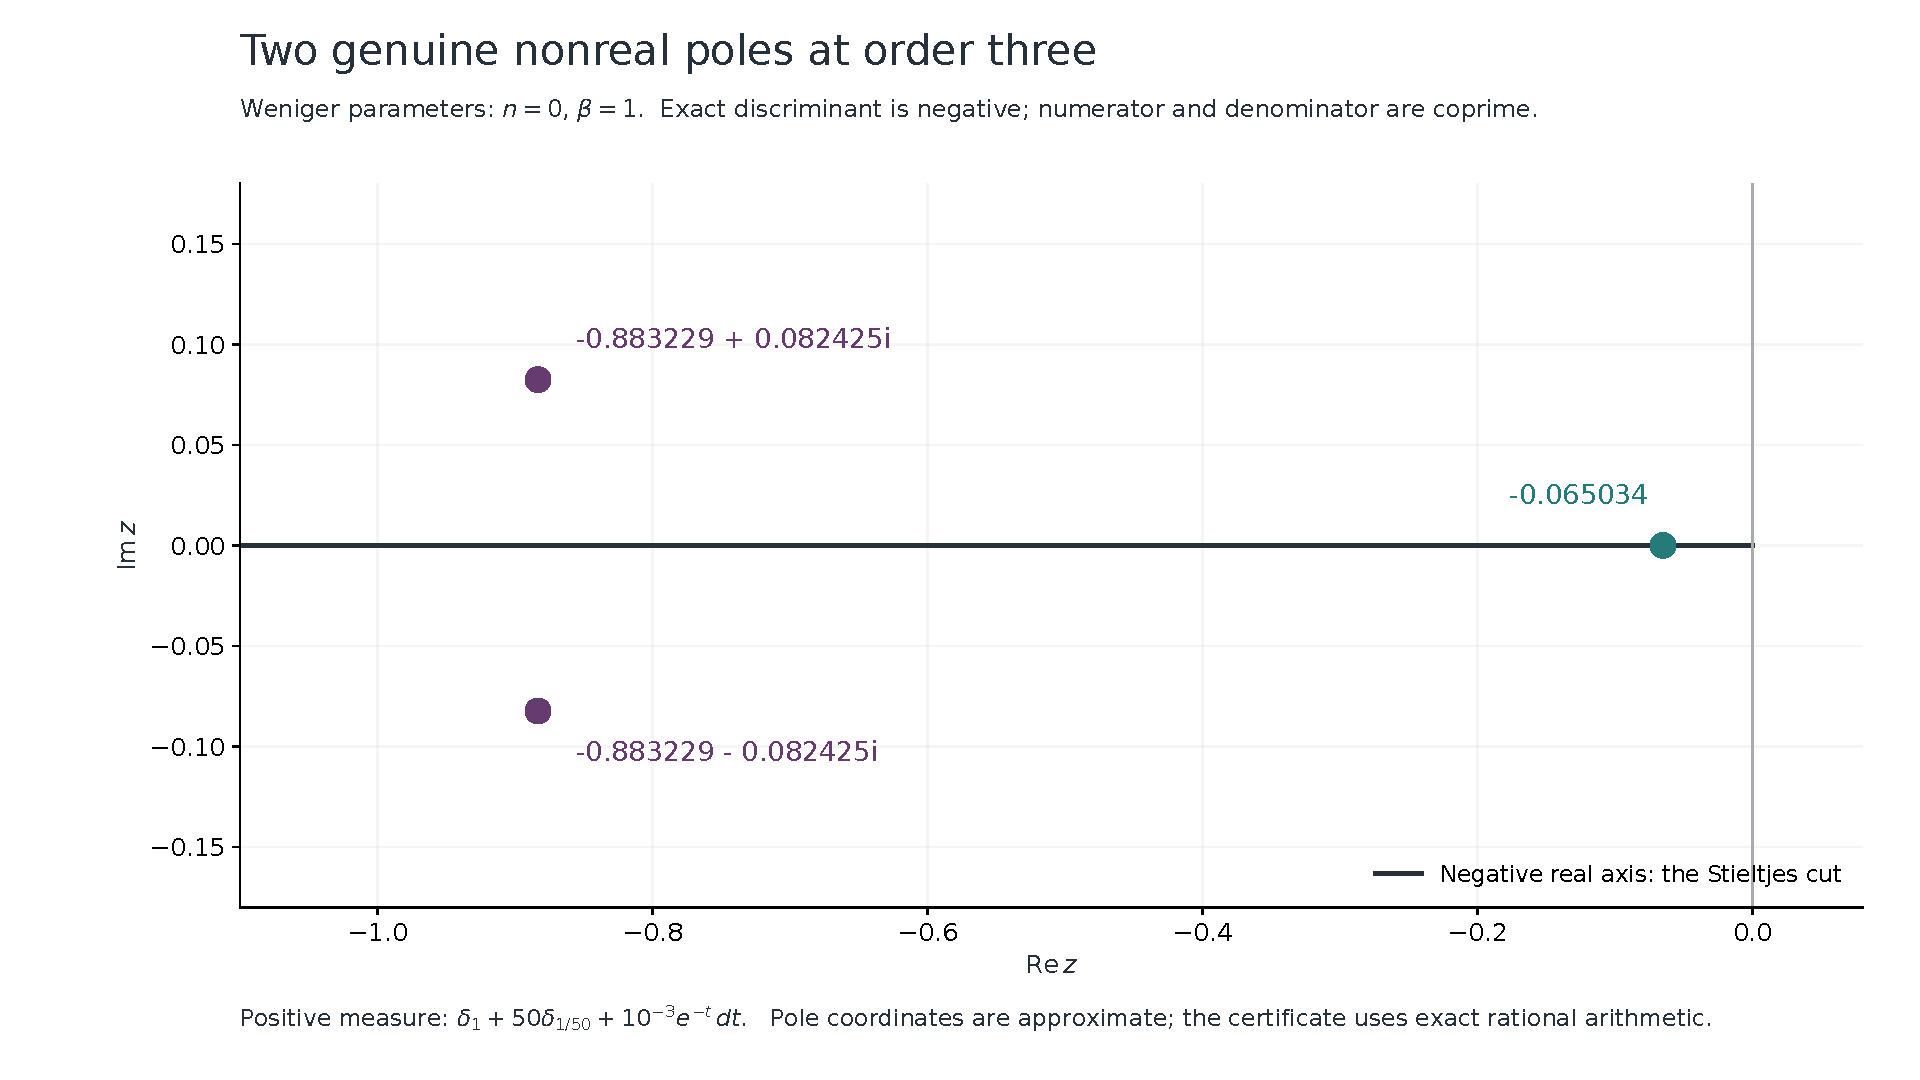
\includegraphics[width=0.9\linewidth]{figures/cubic_nonreal_poles.pdf}
\caption{Poles of $\delta_3^{(0)}(1;z)$ for
$\dd\mu=\dd\delta_1+50\dd\delta_{1/50}+10^{-3}e^{-t}\dd t$: one negative real
pole, the pole at the branch point $z=0$ (not marked; residue about $32.7$, \S\ref{sec:practice}), and a
genuine nonreal pair. Coordinates are floating-point approximations; the
nonreal pair is certified by the exact discriminant.}
\label{fig:poles}
\end{figure}

\paragraph{Order four inside the cubic-safe range.}
For $\dd\lambda=\dd\delta_1+10^5\dd\delta_{1/100}+10^{-3}e^{-t}\dd t$ at $n=0$,
$\beta=1/3<\bc$, every cubic is real-rooted, but the quartic denominator
$\widehat Q_4$ violates the Laguerre inequality
$(q')^2-qq''\ge0$ (valid at every real point for real-rooted $q$, since
$(q')^2-qq''=q^2\sum_r(x-r)^{-2}$): the value at $x=-1$ is a negative
$38$-digit integer. Numerically, the two real zeros lie in $(-0.03,0)$
and the nonreal pair is near $-1.14\pm0.23i$, so $x=-1$ is close to the pair. Exact arithmetic gives
$\delta_4^{(0)}(1/3;z)=3\widehat P_4(z)/(1000z\widehat Q_4(z))$ with
primitive integer polynomials $\widehat P_4,\widehat Q_4$ (listed in the
certificate) and $\gcd(\widehat P_4,\widehat Q_4)=1$.

\paragraph{One input, every shift.}
\begin{proposition}\label{prop:allshift}
For the measure $\lambda$ and every $\beta>0$, $Q_4^{(n,\beta)}$ has exactly
one nonreal conjugate pair of zeros, and it is a genuine pair of poles of
$\delta_4^{(n)}(\beta;\cdot)$, both for $n=0$ and for $n=1$.
\end{proposition}
\begin{proof}
For $n=0$ the discriminant of $Q_4^{(0,\beta)}$, computed over $\mathbb Q[\beta]$
by the 16-term quartic formula and independently by the $7\times7$
Sylvester determinant, is a polynomial of degree $18$ in $\beta$ with all
nineteen coefficients negative; it factors as
$-c(\beta+1)(\beta+2)^2(\beta+4)^2(\beta+5)\,C(\beta)$ with $c>0$ and
$C$ of degree $12$ with positive integer coefficients (listed in the
certificate). For $n=1$ the discriminant, as a polynomial in $\beta$ of
degree $18$, again has only negative coefficients. A negative quartic
discriminant means exactly one nonreal pair; positive coefficients make the
real zeros negative; Proposition~\ref{prop:noncancellation} excludes
cancellation.
\end{proof}
The same measure fails at $n=2$: there the discriminant is positive at
$\beta=0$, and at $\beta=1$ an exact Sturm count shows that
$Q_4^{(2,1)}$ has four real zeros, all negative, so
$\delta_4^{(2)}(1;\cdot)$ has no nonreal poles. The present explicit
measure does not work for every $n$; the following construction permits
the measure to depend on $n$. For each fixed $n$ it gives such a measure,
though without explicit constants.

\begin{corollary}[One quartic measure for all shifts]\label{cor:allshifts}
For every fixed $n\ge0$ there is an admissible measure, with moments
$\sim c\,\ell!$, such that $\delta_4^{(n)}(\beta;\cdot)$ has a genuine nonreal
conjugate pair of poles for every $\beta>0$.
\end{corollary}
\begin{proof}
Take $\mu^{\mathrm{tail}}_K$ of \eqref{eq:tailmeasure} with $k=4$, so
$\ell_0=m+1$ and $\mu_\ell=1+K^{2m+3-2\ell}+K^{-1}\ell!$; it does not depend
on $\beta$. Write $b=n+\beta\in(n,\infty)\subset[0,\infty)$ and divide
$Q_4^{(n,\beta)}$ by its leading coefficient $h_4/\mu_{m+4}$. The resulting
coefficients are $(h_j/h_4)(\mu_{m+4}/\mu_{m+j})$. Here
$0<h_j/h_4\le\binom4j$, since $(b+j)_3\le(b+4)_3$. The moment ratios do not
depend on $b$: they tend to $0$ for $j=0,1$ (as $\mu_m,\mu_{m+1}\ge K$) and
to $1$ for $j=2,3,4$. Hence the normalised denominator converges to
$z^2g_b(z)$, coefficientwise and uniformly in $b\ge0$, where
\[
 g_b(z)=z^2+\frac{4(b+3)}{b+6}z+\frac{6(b+2)(b+3)}{(b+5)(b+6)},\qquad
 \Disc(g_b)=-\frac{8(b+3)(b^2+8b+6)}{(b+5)(b+6)^2}\le-\frac45 ;
\]
the inequality is $10(b+3)(b^2+8b+6)-(b+5)(b+6)^2=9b^3+93b^2+204b\ge0$.
The zeros of $g_b$ are $w_b,\bar w_b$ with
$\operatorname{Re}w_b=-2(b+3)/(b+6)\in[-2,-1]$ and
$\operatorname{Im}w_b=\tfrac12\sqrt{-\Disc(g_b)}\ge1/\sqrt5$. On the circle
$|z-w_b|=\rho:=1/(2\sqrt5)$ we have $|z|\ge1-\rho$ and
$|z-\bar w_b|\ge2/\sqrt5-\rho$, so
$|z^2g_b(z)|\ge(1-\rho)^2\rho(2/\sqrt5-\rho)=:\varepsilon>0$, uniformly in
$b$. All these circles lie in $|z|\le3$, where the difference between the
normalised denominator and $z^2g_b$ is at most $3^4\cdot5$ times the largest
coefficient error, which tends to $0$ uniformly in $b$. Fix $K$ so large that
this bound is below $\varepsilon$. By Rouché's theorem, for every $b\ge0$ the
denominator has a zero in the disk $|z-w_b|<\rho$, which lies in the upper
half-plane, together with its conjugate. Proposition~\ref{prop:noncancellation}
excludes cancellation of a nonreal pair at order four, for every $\beta$.
The moments satisfy $\mu_\ell\sim K^{-1}\ell!$.
\end{proof}

\paragraph{Explicit sizes for orders five to eight.}
Table~\ref{tab:tail} replaces the limit $K\to\infty$ in
\eqref{eq:tailmeasure} by explicit values: for each case the smallest
$K=2^e$ ($e\le16$) is listed at which an exact Sturm count shows nonreal
zeros of $Q_k$ and exact Euclidean division shows $\gcd(P_{n,k},Q_k)=1$. No
perturbation is needed.

\begin{table}[htbp]
\centering
\caption{Certified genuine nonreal poles from $\mu^{\mathrm{tail}}_K$,
eq.~\eqref{eq:tailmeasure}: smallest $K=2^e$, and the number of nonreal
zeros of $Q_k$.}
\label{tab:tail}
\small
\begin{tabular}{@{}ccccccc@{}}
\toprule
& \multicolumn{3}{c}{$n=0$} & \multicolumn{3}{c}{$n=1$}\\
\cmidrule(lr){2-4}\cmidrule(lr){5-7}
$k$ & $\beta=1/10$ & $\beta=1$ & $\beta=5$ & $\beta=1/10$ & $\beta=1$ & $\beta=5$\\
\midrule
5 & $2^{11}$ (2) & $2^{10}$ (2) & $2$ (2) & $4$ (2) & $4$ (2) & $2$ (2)\\
6 & $4$ (2) & $4$ (2) & $2$ (4) & $2$ (2) & $2$ (2) & $2$ (2)\\
7 & $2$ (2) & $2$ (2) & $2$ (4) & $2$ (2) & $2$ (2) & $2$ (4)\\
8 & $2$ (2) & $2$ (4) & $2$ (4) & $2$ (2) & $2$ (4) & $2$ (6)\\
\bottomrule
\end{tabular}
\end{table}

\begin{remark}[Borghi's scenario (ii)]\label{rem:scenario}
In every counterexample of this paper Borghi's polynomial $P_k$ has
nonreal zeros (exact Sturm counts: $2$ for the cubic and quartic examples,
$2$--$6$ in Table~\ref{tab:tail}). This must be so: by
Theorem~\ref{thm:positive}(a) below, real-rooted $P_k$ forces real-rooted
$Q_k$. The counterexamples therefore lie exactly in the case his
Gauss--Lucas argument leaves open, and show that the open case can fail.
It need not fail. Borghi already shows this numerically: his Fig.~1
\cite[\S4.6]{Borghi2026} displays, for a Jacobi weight whose parameters do
not differ by an integer ($k=20$), a $P_k$ with nonreal zeros and a $Q_k$
with only real zeros. The non-integer Jacobi tests in \S\ref{sec:positive}
show the same behaviour at other $(k,n,\beta)$.
\end{remark}

\section{One fixed measure at all large orders}\label{sec:persistence}

Theorem~\ref{thm:main} lets the measure depend on the order. Here we fix
the measure.

\begin{theorem}[Small-scale limit]\label{thm:limit}
Let $\mu$ be admissible, $n\ge0$, $\beta>0$. Define
\begin{equation}\label{eq:E}
 E_\mu(w)=\sum_{j\ge0}\frac{w^j}{j!\,(b)_j\,\mu_{m+j}} .
\end{equation}
Then $E_\mu$ is entire of order at most $1/2$, and
$(b)_{k-1}^{-1}Q_k^{(n,\beta)}(w/k^2)\to E_\mu(w)$ uniformly on compact
subsets of $\mathbb C$ as $k\to\infty$.
\end{theorem}
\begin{proof}
Using $(b+j)_{k-1}/(b)_{k-1}=(b+k-1)_j/(b)_j$,
\[
 \frac{Q_k(w/k^2)}{(b)_{k-1}}=\sum_{j=0}^k t_{k,j}\frac{w^j}{j!(b)_j\mu_{m+j}},
 \qquad t_{k,j}=\prod_{i=0}^{j-1}\Bigl(1-\frac ik\Bigr)\Bigl(1+\frac{b-1+i}{k}\Bigr).
\]
For $1\le i<k$ the factor equals $1+(b-1)/k-i(b-1+i)/k^2\in[0,1+|b-1|]$
(note $b-1+i\ge b>0$), and it equals $1+(b-1)/k$ for $i=0$; so
$0\le t_{k,j}\le(1+|b-1|)^j$ and $t_{k,j}\to1$ for fixed $j$. By
\eqref{eq:logconvex}, $\mu_{m+j}\ge\mu_m(\mu_{m+1}/\mu_m)^j$, so the
coefficients of $E_\mu$ are at most $C\theta^j/(j!(b)_j)$; this gives order
at most $1/2$ and a summable majorant on every disk, and the Weierstrass
M-test gives locally uniform convergence.
\end{proof}

\begin{corollary}\label{cor:hurwitz}
Let $\mu$, $n$, $\beta$ be fixed.
\begin{enumerate}
\item If $E_\mu$ has a nonreal zero, there is $k_0$ such that
$Q_k^{(n,\beta)}$ has a nonreal zero for every $k\ge k_0$; these zeros are
asymptotic to $w^*/k^2$ for a nonreal zero $w^*$ of $E_\mu$.
\item If $Q_k^{(n,\beta)}$ is real-rooted for infinitely many $k$, then
$E_\mu$ belongs to the Laguerre--Pólya class.
\item $E_\mu$ has a nonreal zero as soon as one Jensen polynomial
$g_d(w)=\sum_{j=0}^d\binom dj w^j/\bigl((b)_j\mu_{m+j}\bigr)$ has a nonreal zero.
\end{enumerate}
\end{corollary}
\begin{proof}
1 and 2 follow from Theorem~\ref{thm:limit} and Hurwitz's theorem
(the Laguerre--Pólya class is closed under locally uniform limits of
real-rooted polynomials). For 3: a real entire function of order
$<2$ with only real zeros is, by Hadamard's theorem, in the
Laguerre--Pólya class, and then all its Jensen polynomials are real-rooted
\cite{PolyaSchur1914}, \cite[\S1]{CravenCsordas1989}.
\end{proof}

\begin{theorem}[Persistence for one measure]\label{thm:persist}
Let $\dd\mu=\dd\delta_1+50\dd\delta_{1/50}+10^{-3}e^{-t}\dd t$, $n=0$, $\beta=1$.
\begin{enumerate}
\item For every $3\le k\le30$, $Q_k^{(0,1)}$ has nonreal zeros and
$\gcd(P_{0,k},Q_k)=1$; so $\delta_k^{(0)}(1;\cdot)$ has genuine nonreal poles.
The numbers of nonreal zeros are given in Table~\ref{tab:persist}.
\item There is $k_0$ such that $Q_k^{(0,1)}$ has nonreal zeros for every
$k\ge k_0$. In particular nonreal denominator zeros occur at infinitely
many orders.
\end{enumerate}
\end{theorem}
\begin{proof}
Part 1 is an exact Sturm-sequence count and an exact gcd at each order
(certificate, section \texttt{D}). For part 2, here
$E_\mu(w)=\sum_j w^j/\bigl((j!)^2\mu_{j+1}\bigr)$, and the Jensen polynomial
$g_6(w)=\sum_{j=0}^6\binom6jw^j/(j!\,\mu_{j+1})$ has exactly two nonreal
zeros by an exact Sturm count ($g_1,\dots,g_5$ are real-rooted). Apply
Corollary~\ref{cor:hurwitz}.
\end{proof}

\begin{table}[htbp]
\centering
\caption{Exact numbers of nonreal zeros of $Q_k^{(0,1)}$ (row $Q$) and of
Borghi's $P_k$ (row $P$) for the measure of Theorem~\ref{thm:persist}; in
every case $\gcd(P_{0,k},Q_k)=1$.}
\label{tab:persist}
\scriptsize
\setlength{\tabcolsep}{3.2pt}
\begin{tabular}{@{}l*{14}{c}@{}}
\toprule
$k$ & 3 & 4--7 & 8 & 9 & 10 & 11--12 & 13--14 & 15--17 & 18--19 & 20 & 21--23 & 24--29 & 30\\
\midrule
$Q$ & 2 & 2 & 4 & 4 & 4 & 6 & 6 & 8 & 8 & 10 & 10 & 10 & 10\\
$P$ & 2 & 2 & 4 & 6 & 8 & 8 & 10 & 12 & 14 & 14 & 16 & 18 & 20\\
\bottomrule
\end{tabular}
\end{table}

Numerically, $E_\mu$ has the zero $w^*\approx-9.1021+9.1273\,i$, and the
zero of $Q_k$ closest to $w^*/k^2$ satisfies $k^2z\approx-10.12+8.04i$,
$-9.38+8.88i$, $-9.23+9.02i$ at $k=10,20,30$. This nonreal pair of
denominator zeros thus approaches the branch point $z=0$ at rate $k^{-2}$
(it is certified to give genuine poles only for $k\le30$). The proof of part~2 is
not effective: it does not give $k_0$, so we do not close the gap. Nor does
Proposition~\ref{prop:noncancellation} exclude cancellation at large $k$.

\begin{conjecture}\label{conj:persist}
For the measure of Theorem~\ref{thm:persist}, $\delta_k^{(0)}(1;\cdot)$ has
genuine nonreal poles at every order $k\ge3$.
\end{conjecture}

The evidence is Table~\ref{tab:persist}, part 2 of the theorem, and the
convergence of the scaled zeros to $w^*$.

\section{A positive theorem and natural families}\label{sec:positive}

\begin{lemma}[Rolle step]\label{lem:rolle}
Let $f$ be a real polynomial of degree $d$ with positive coefficients and
only real zeros, and $c>0$. Then $zf'(z)+cf(z)$ has degree $d$ and only
negative real zeros.
\end{lemma}
\begin{proof}
For $x<0$ put $g(x)=(-x)^cf(x)$; then
$g'(x)=-(-x)^{c-1}\bigl(xf'(x)+cf(x)\bigr)$. Let $f$ have distinct zeros
$s_1<\dots<s_p<0$ with multiplicities summing to $d$. A zero of
multiplicity $r$ of $f$ is a zero of multiplicity $r-1$ of $xf'+cf$. Rolle's
theorem gives a zero of $g'$ in each $(s_i,s_{i+1})$ and one in $(s_p,0)$,
because $g(s_p)=0=g(0^-)$. This accounts for $d$ zeros, all negative.
\end{proof}

Recall that a real sequence $(\gamma_j)_{j\ge0}$ is a \emph{multiplier
sequence} if $\sum\gamma_ja_jz^j$ is real-rooted whenever $\sum a_jz^j$ is.
By Pólya and Schur \cite{PolyaSchur1914} (see \cite{CravenCsordas1989}), a
positive sequence is a multiplier sequence if and only if
$\sum_{j\le k}\binom kj\gamma_jz^j$ is real-rooted for every $k$.

\begin{theorem}[Positive criteria]\label{thm:positive}
Fix $n\ge0$, $m=n+1$, $k\ge1$ and an admissible measure.
\begin{enumerate}
\item[(a)] If Borghi's $P_k$ in \eqref{eq:borghiP} has only real zeros,
then $Q_k^{(n,\beta)}$ has only negative real zeros for every $\beta>0$.
\item[(b)] If $(1/\mu_{m+j})_{j\ge0}$ is a multiplier sequence (equivalently,
$P_k$ is real-rooted for every $k$), then $Q_k^{(n,\beta)}$ has only negative
real zeros for every $k\ge1$ and $\beta>0$.
\item[(c)] If $\mu_{r-1}\mu_{r+1}\ge4\mu_r^2$ for $m+1\le r\le m+k-1$, then
$Q_k^{(n,\beta)}$ has $k$ distinct negative zeros for every $\beta>0$.
\end{enumerate}
\end{theorem}
\begin{proof}
(a) With $\vartheta=z\,\mathrm d/\mathrm dz$ we have
$(\vartheta+c)z^j=(j+c)z^j$, so
$Q_k=\prod_{i=0}^{k-2}(\vartheta+b+i)\,P_k$; apply Lemma~\ref{lem:rolle}
$k-1$ times. This is Borghi's identity
$Q_k=z^{1-b}\frac{\mathrm d^{k-1}}{\mathrm dz^{k-1}}[z^{b+k-2}P_k]$ in operator form, and
it extends his scenario (i) to every $n$ and $\beta$ (non-integer
exponents need Lemma~\ref{lem:rolle}).
(b) follows from (a) and the Pólya--Schur characterisation.
(c) For the delta weights,
\[
 \frac{h_j^2}{h_{j-1}h_{j+1}}=\frac{(j+1)(k-j+1)}{j(k-j)}
 \Bigl(1+\frac{k-1}{(s-1)(s+k-1)}\Bigr)>1,\qquad s=b+j>1,
\]
so the coefficient ratios of $Q_k$ exceed $4$; apply Lemma~\ref{lem:four}.
\end{proof}

\begin{corollary}[Natural families]\label{cor:families}
$Q_k^{(n,\beta)}$ has only negative real zeros for every $k$, $n$ and
$\beta>0$ in each of the following cases.
\begin{enumerate}
\item $\mu_\ell=\Gamma(\ell+a)$, $a>0$: the Euler series ($a=1$),
$\Gamma(\ell+1/2)$, $\Gamma(\ell+5)$, and Borghi's Laguerre distribution
\cite[\S4.3]{Borghi2026}. Here $P_k(z)=\frac{k!}{\Gamma(m+a+k)}L_k^{(m+a-1)}(-z)$,
and Laguerre polynomials with parameter $>-1$ have positive simple zeros
\cite[Thm.~3.3.1]{Szego1939}. With $a=1$, $n=0$, $\beta=1$ this recovers the
real-rootedness of the Euler-series denominator quoted by Borghi from
\cite[Thm.~5.1]{BorghiWeniger2015}.
\item $\mu_\ell=\Gamma(\nu\ell+c)$ with integer $\nu\ge1$ and $c>0$, for
example $(2\ell)!$ and $(3\ell)!$.
\item Beta (Jacobi-type) weights $t^\alpha(1-t)^{p}$ on $[0,1]$ with
$\alpha>-1$ and integer $p\ge0$, including $\mu_\ell=1/(\ell+1)$.
\item Log-normal moments $\mu_\ell=e^{\sigma^2\ell^2/2}$ with
$\sigma^2\ge2\log2$ (distinct zeros).
\end{enumerate}
\end{corollary}
\begin{proof}
1: by (a) of Theorem~\ref{thm:positive} for every $k$; in particular
$(1/\Gamma(j+a'))_j$ is a multiplier sequence for every $a'>0$.
2: Gauss's multiplication formula gives
$1/\mu_{m+j}=C\nu^{-\nu j}\prod_{i=0}^{\nu-1}1/\Gamma\bigl(j+m+(c+i)/\nu\bigr)$, a
termwise product of multiplier sequences, hence a multiplier sequence;
apply (b). 3: $1/\mu_{m+j}$ is a positive constant times
$(\alpha+m+1+j)_{p+1}$, a polynomial in $j$ with negative zeros, so
$P_k=\prod_{i=0}^{p}(\vartheta+\alpha+m+1+i)(1+z)^k$ up to a constant, which is
real-rooted by Lemma~\ref{lem:rolle}; apply (a). 4: the moment ratio equals
$e^{\sigma^2}\ge4$; apply (c).
\end{proof}

At Borghi's normalisation $n=0$, $\beta=1$, the cases of items 1--3 are due
to him, except item 2 with $c\ge2$: he proves
real-rootedness of $P_k$, and hence of $Q_k$, for the superfactorial
moments $\Gamma(\nu\ell+q+1)$ with integer $\nu$ and $q\in(-1,1)$ through
Pólya frequency functions \cite[\S4.2]{Borghi2026}, for the Laguerre
distribution as a special case \cite[\S4.3]{Borghi2026}, and for Jacobi
weights whose parameters differ by an integer \cite[\S4.6]{Borghi2026}
(our item 3). What is new in Corollary~\ref{cor:families} is the
extension to every $n$, $\beta$ and $k$ (and to every $c>0$ in item 2),
obtained by one proof through Theorem~\ref{thm:positive}. The limit function of \S\ref{sec:persistence} is consistent with
this picture: when $(1/\mu_{m+j})$ is a multiplier sequence, $E_\mu$ is in the
Laguerre--Pólya class.

\paragraph{Exact tests.}
The certificate (section \texttt{F}) counts real zeros exactly for
$4\le k\le8$, $n\in\{0,1,2\}$ and $\beta\in\{1/10,1/2,1,2,5\}$ ($975$ Sturm
counts) for: $\ell!$, $(2\ell)!$, $(3\ell)!$, $\Gamma(\ell+1/2)$,
$\Gamma(\ell+5)$, $1/(\ell+1)$, log-normal $2^{\ell^2}$, the
Weniger--Čížek moments $\mu_\ell=(\tfrac12+\nu)_\ell(\tfrac12-\nu)_\ell/(2^\ell\ell!)$
of $K_\nu$ \cite{WenigerCizek1990} for $\nu\in\{0,1/4,1/3\}$ (Borghi's eq.~(47)
case, for which he reports no proof), and Jacobi weights with
$(\alpha,p)\in\{(-\tfrac12,\tfrac12),(\tfrac12,-\tfrac12),(\tfrac13,\tfrac23)\}$.
Every $Q_k$ on this grid is real-rooted. For the $K_\nu$ and Jacobi cases
this is evidence, not proof, and only for the tested shifts
$\beta\le5$; for the three non-integer Jacobi weights
Borghi's $P_k$ has nonreal zeros at every tested $(k,n)$, so these are
real-rooted cases inside scenario (ii), as in Borghi's Fig.~1. By
Remark~\ref{rem:largeshift} they cannot stay real-rooted for every shift.

\begin{remark}[Large shifts]\label{rem:largeshift}
Fix $n$, $k$ and an admissible measure. Then
$\beta^{-(k-1)}Q_k^{(n,\beta)}(z)\to P_k(z)$ as $\beta\to\infty$, so
$Q_k^{(n,\beta)}$ is real-rooted for every $\beta>0$ if and only if $P_k$
is real-rooted.
\end{remark}
\begin{proof}
With $b=n+\beta$, the coefficient of $z^j$ in $\beta^{-(k-1)}Q_k$ is
$\binom kj\bigl((b+j)_{k-1}/\beta^{k-1}\bigr)/\mu_{m+j}$, and
$(b+j)_{k-1}/\beta^{k-1}=\prod_{i=0}^{k-2}\bigl(1+(n+j+i)/\beta\bigr)\to1$.
So the coefficients converge to those of $P_k$, and the degree stays $k$
with leading coefficient bounded away from $0$. If $P_k$ has a nonreal
zero $z^*$, Hurwitz's theorem on a small disk about $z^*$ in the open
half-plane gives a nonreal zero of $Q_k^{(n,\beta)}$ for all large $\beta$.
Conversely, the zeros of $Q_k^{(n,\beta)}$ converge to those of $P_k$ with
multiplicity, so $P_k$ is real-rooted if $Q_k^{(n,\beta)}$ is real-rooted
along a sequence $\beta\to\infty$. The reverse implication is
Theorem~\ref{thm:positive}(a).
\end{proof}
For the Jacobi weight $t^{-1/2}(1-t)^{1/2}$, $n=0$, $k=4$ and $\beta=20$,
outside the tested grid, the primitive denominator is
$416000z^4+1104000z^3+1020096z^2+371910z+40425$; its discriminant is
negative, an exact Sturm count gives two nonreal zeros, and
$\gcd(P_{0,4},Q_4)=1$, so these are genuine nonreal poles (certificate,
section \texttt{F}).

\section{Practical consequences}\label{sec:practice}

The figures in this section are floating-point computations (mpmath,
60 digits) and are illustrative; only the counts of nonreal zeros and the
gcd degrees are exact.

\paragraph{Where the poles sit and what they do.}
In the cubic example (Figure~\ref{fig:poles}) the nonreal pair
$-0.8832\pm0.0824i$ lies close to the cut and has residues
$0.357\pm1.360i$, of modulus about $1.4$; the real poles at $-0.0650$ and
$0$ have positive residues $17.6$ and $32.7$. These are not small
Froissart-type residues, and they are not positive, so $\delta_3$ is not
itself a Stieltjes function, unlike every Padé approximant
\cite[Ch.~5]{BakerGM1996}. The relative error of $\delta_3$ is
$1.1\times10^{-8}$ at $z=10$, $1.1\times10^{-4}$ at $z=1$,
$2.9\times10^{-4}$ at $z=i$, $3.9\times10^{-2}$ at $z=0.1$ and
$1.3\times10^{-2}$ at $z=-0.5+0.3i$: the defect is local to the region near
the cut. In the persistence example the nonreal denominator zeros move to
the branch point like $k^{-2}$; they are certified genuine poles for
$3\le k\le30$ only.

\paragraph{Accuracy co-occurrence.}
For $f(z)=100/(z+2)+\int_0^\infty e^{-t}(z+t)^{-1}\dd t$ (moments
$100\cdot2^\ell+\ell!$; a continuum plus one pole), $n=0$, $\beta=1$:
\begin{center}
\small
\begin{tabular}{@{}lccccccccc@{}}
\toprule
$k$ & 2 & 4 & 8 & 12 & 16 & 20 & 30 & 40 & 50\\
\midrule
relative error at $z=1$ & $1.8\mathrm{e}{-3}$ & $1.5\mathrm{e}{-2}$ & $0.43$ & $1.55$ & $1.52$ & $0.98$ & $0.43$ & $4.5\mathrm{e}{-2}$ & $9.5\mathrm{e}{-3}$\\
nonreal zeros of $Q_k$ (exact) & 0 & 0 & 2 & 4 & 8 & 10 & 14 & 16 & 18\\
\bottomrule
\end{tabular}
\end{center}
with $\gcd(P_{0,k},Q_k)=1$ in every case, while the pure Euler series has
errors $2.2\times10^{-7}$ ($k=8$) and $6.5\times10^{-18}$ ($k=30$). The
error transient and the nonreal poles occur together; we make no causal
claim, since the poles stay at distance of order one from $z=1$.

\paragraph{A diagnostic.}
For given data, real-rootedness of the computed $Q_k$ can be decided exactly:
clear denominators and count real zeros with a Sturm sequence (or the sign
of the discriminant at $k\le4$); decide genuineness with an exact gcd. The
function \texttt{real\_root\_count} in \texttt{code/verify\_all.py} does
this in rational arithmetic. The factor-four test of
Lemma~\ref{lem:four} is \emph{not} a useful diagnostic: for the Euler
moments at $n=0$, $\beta=1$, $k=10$ its smallest ratio is $1.82<4$, yet
$Q_{10}$ is real-rooted. It is a sufficient condition only.

\section{Scope and open problems}\label{sec:scope}

The classification concerns pole location at fixed finite order for the
worst case over all admissible measures. It says nothing against the
convergence results for special families \cite{BorghiWeniger2015,
Borghi2026asymptotic}, and Section~\ref{sec:positive} shows
that those families are real-rooted at every order. These results rule
out an argument requiring the unreduced delta denominator to be
real-rooted at all sufficiently large orders. Persistence of genuine
nonreal poles for the fixed measure remains open beyond the certified
orders ($3\le k\le30$; Conjecture~\ref{conj:persist}). The practical lesson is that, for Stieltjes series of mixed
character (for example a continuum plus isolated poles), real-rootedness of
the delta denominator should be checked rather than assumed.

Open problems: (i) prove Conjecture~\ref{conj:persist}, including
genuineness at large orders; (ii) characterise the measures for which
$E_\mu$ lies in the Laguerre--Pólya class, and decide whether this is also
sufficient for real-rootedness at all large orders; (iii) decide the
Weniger--Čížek $K_\nu$ family; (iv) treat other Levin-type weights, such
as Levin's $t$ and $u$ transformations.

\appendix
\section{The cubic boundary by discriminants}\label{app:cubic}

With $m=n+1$, set $\gamma=\mu_{m+1}/\mu_m$ and normalised moments
$\rho_r=\mu_{m+r}/(\mu_m\gamma^r)$, so $(\rho_0,\dots,\rho_3)=(1,1,u,u^2v)$ with
$u=\mu_m\mu_{m+2}/\mu_{m+1}^2\ge1$, $v=\mu_{m+1}\mu_{m+3}/\mu_{m+2}^2\ge1$.
With $x=1/u$, $y=1/v$ and $D,C,B,A$ as in \S\ref{sec:cubic},
\[
 p(\zeta):=\mu_mQ_3(\gamma\zeta)=D+C\zeta+Bx\zeta^2+Ax^2y\zeta^3,\qquad0<x,y\le1 .
\]
Using $\Disc(e_3\zeta^3+e_2\zeta^2+e_1\zeta+e_0)=e_2^2e_1^2-4e_3e_1^3-4e_2^3e_0
-27e_3^2e_0^2+18e_3e_2e_1e_0$,
\begin{equation}\label{eq:disc}
 \Disc(p)=x^2F(x,y),\qquad
 F=B^2C^2-4AC^3y+x(-4B^3D+18ABCDy)-27A^2D^2x^2y^2 .
\end{equation}
(The certificate verifies \eqref{eq:disc} as an identity in $\mathbb Q[b,x,y]$.)
$F$ is concave in $x$ for fixed $y$ and in $y$ for fixed $x$, so
$F(x,y)\ge(1-x)(1-y)F(0,0)+(1-x)yF(0,1)+x(1-y)F(1,0)+xyF(1,1)$, with
$F(0,0)=B^2C^2$, $F(0,1)=C^2(B^2-4AC)$, $F(1,0)=B^2(C^2-4BD)$ and
$F(1,1)=432(b+1)(b+3)$ (the last from
$D+C\zeta+B\zeta^2+A\zeta^3=(1+\zeta)[A\zeta^2+2(b+1)(b+3)\zeta+D]$). For
$b\le\bc$ all four are nonnegative and the last positive, so
$F\ge xyF(1,1)>0$ and $p$ has three distinct negative zeros; this includes
$b=\bc$ and non-strict log-convex quadruples.

For $b>\bc$, $F(0,1)<0$. The admissible family
$\dd\mu^{\mathrm{cub}}_K=\dd\delta_1+K^{2m+1}\dd\delta_{K^{-2}}+K^{-1}e^{-t}\dd t$,
$\mu_\ell=1+K^{2m+1-2\ell}+K^{-1}\ell!$, has $\mu_m\sim K$ and
$\mu_{m+1},\mu_{m+2},\mu_{m+3}\to1$, so $(x,y)\to(0,1)$ and $F<0$ for large
$K$. The certificate lists the first $K=2^e$ that works for four
parameter pairs (for example $K=128$ at $n=0$, $\beta=1$, and $K=4096$ at
$n=0$, $\beta=2/5$, close to the threshold).

\section{Reproducibility}\label{app:repro}

The package is archived at \url{https://doi.org/10.5281/zenodo.23586255}; the repository is
\url{https://github.com/ipitchford/weniger-delta-nonreal-poles} (tag \texttt{v1.0.0-candidate}).
It contains \texttt{code/verify\_all.py} (Python~3; exact parts
use only the standard library, the illustrative \texttt{numerical\_*}
sections use mpmath). Run
\begin{verbatim}
python3 -B -O code/verify_all.py results
\end{verbatim}
It writes \texttt{results/verification.json} with sorted keys, no
timestamps or paths, and floats rounded to eight significant figures, and
stops with an error if any exact check fails. It checks: the corner
identities and the discriminant identity \eqref{eq:disc} over
$\mathbb Q[b,x,y]$; identity \eqref{eq:DeltaQ} coefficientwise over
$\mathbb Q[b]$ for $n\le3$, $k\le8$; \eqref{eq:tailratio} over $\mathbb Q[b]$
for $3\le k\le12$; the rational form \eqref{eq:rational} against the
definition \eqref{eq:delta} at $81$ rational points; the explicit cubic and
quartic examples (discriminants, Laguerre value, gcds, resultants,
accuracy); the Legendre integrals; the cubic sharpness family; the
all-shift identities of Proposition~\ref{prop:allshift}, the four real zeros
of $Q_4^{(2,1)}$ for $\lambda$, and the identities for $g_b$ in
Corollary~\ref{cor:allshifts}; the factorisation $(k-4)(4k-5)$ in
\eqref{eq:tailbound}; the persistence
certificate of Theorem~\ref{thm:persist} including the Jensen polynomials
$g_1,\dots,g_{12}$; Table~\ref{tab:tail}; and the natural-family tests and
the Laguerre identity, including its constant, and the large-shift Jacobi
example of \S\ref{sec:positive}. Finite checks supplement
the proofs; they do not replace the all-parameter arguments.

\begin{thebibliography}{99}\small\sloppy

\bibitem{BakerGM1996}
G.~A. Baker, Jr. and P.~Graves-Morris, \emph{Padé Approximants}, 2nd ed.,
Cambridge University Press, 1996.
\href{https://doi.org/10.1017/CBO9780511530074}{doi:10.1017/CBO9780511530074}.

\bibitem{Borghi2026}
R.~Borghi, Is Weniger's transformation capable of simulating the Stieltjes
function branch cut?, \emph{Mathematics} \textbf{14} (2026), no.~2, 376.
\href{https://doi.org/10.3390/math14020376}{doi:10.3390/math14020376}.

\bibitem{Borghi2026asymptotic}
R.~Borghi, Asymptotic convergence of Weniger's $\delta$-transformation for
a class of superfactorially divergent Stieltjes series, preprint (2026),
\href{https://arxiv.org/abs/2605.06687}{arXiv:2605.06687}.

\bibitem{BorghiWeniger2015}
R.~Borghi and E.~J. Weniger, Convergence analysis of the summation of the
factorially divergent Euler series by Padé approximants and the delta
transformation, \emph{Appl. Numer. Math.} \textbf{94} (2015), 149--178.
\href{https://doi.org/10.1016/j.apnum.2015.03.007}{doi:10.1016/j.apnum.2015.03.007}.

\bibitem{BrezinskiRZ1991}
C.~Brezinski and M.~Redivo-Zaglia, \emph{Extrapolation Methods: Theory and
Practice}, North-Holland, Amsterdam, 1991.

\bibitem{CravenCsordas1989}
T.~Craven and G.~Csordas, Jensen polynomials and the Turán and Laguerre
inequalities, \emph{Pacific J. Math.} \textbf{136} (1989), 241--260.
\href{https://doi.org/10.2140/pjm.1989.136.241}{doi:10.2140/pjm.1989.136.241}.

\bibitem{Homeier2000}
H.~H.~H. Homeier, Scalar Levin-type sequence transformations, \emph{J.
Comput. Appl. Math.} \textbf{122} (2000), 81--147.
\href{https://doi.org/10.1016/S0377-0427(00)00359-9}{doi:10.1016/S0377-0427(00)00359-9}.

\bibitem{Hutchinson1923}
J.~I. Hutchinson, On a remarkable class of entire functions, \emph{Trans.
Amer. Math. Soc.} \textbf{25} (1923), 325--332.
\href{https://doi.org/10.1090/S0002-9947-1923-1501248-1}{doi:10.1090/S0002-9947-1923-1501248-1}.

\bibitem{KostovShapiro2013}
V.~P. Kostov and B.~Shapiro, Hardy--Petrovitch--Hutchinson's problem and
partial theta function, \emph{Duke Math. J.} \textbf{162} (2013), 825--861.
\href{https://doi.org/10.1215/00127094-2087264}{doi:10.1215/00127094-2087264}.

\bibitem{Kurtz1992}
D.~C. Kurtz, A sufficient condition for all the roots of a polynomial to be
real, \emph{Amer. Math. Monthly} \textbf{99} (1992), 259--263.
\href{https://doi.org/10.1080/00029890.1992.11995845}{doi:10.1080/00029890.1992.11995845}.

\bibitem{Levin1973}
D.~Levin, Development of non-linear transformations for improving
convergence of sequences, \emph{Int. J. Comput. Math. B} \textbf{3} (1973),
371--388.
\href{https://doi.org/10.1080/00207167308803075}{doi:10.1080/00207167308803075}.

\bibitem{Passare2011}
M.~Passare, J.~M. Rojas and B.~Shapiro, New multiplier sequences via
discriminant amoebae, \emph{Moscow Math. J.} \textbf{11} (2011), 547--560.
\href{https://arxiv.org/abs/1001.4076}{arXiv:1001.4076}.

\bibitem{PolyaSchur1914}
G.~Pólya and J.~Schur, Über zwei Arten von Faktorenfolgen in der Theorie
der algebraischen Gleichungen, \emph{J. Reine Angew. Math.} \textbf{144}
(1914), 89--113.
\href{https://doi.org/10.1515/crll.1914.144.89}{doi:10.1515/crll.1914.144.89}.

\bibitem{Schmudgen2017}
K.~Schmüdgen, \emph{The Moment Problem}, Graduate Texts in Mathematics 277,
Springer, 2017.
\href{https://doi.org/10.1007/978-3-319-64546-9}{doi:10.1007/978-3-319-64546-9}.

\bibitem{Sidi2003}
A.~Sidi, \emph{Practical Extrapolation Methods}, Cambridge University
Press, 2003.
\href{https://doi.org/10.1017/CBO9780511546815}{doi:10.1017/CBO9780511546815}.

\bibitem{Sidi1981}
A.~Sidi, A new method for deriving Padé approximants for some
hypergeometric functions, \emph{J. Comput. Appl. Math.} \textbf{7} (1981),
37--40.
\href{https://doi.org/10.1016/0771-050X(81)90006-1}{doi:10.1016/0771-050X(81)90006-1}.

\bibitem{Slevinsky2025}
R.~M. Slevinsky, Fast and stable rational approximation of generalized
hypergeometric functions, \emph{Numer. Algorithms} \textbf{98} (2025),
587--624.
\href{https://doi.org/10.1007/s11075-024-01808-w}{doi:10.1007/s11075-024-01808-w}.

\bibitem{Szego1939}
G.~Szegő, \emph{Orthogonal Polynomials}, AMS Colloquium Publications 23,
1939.
\href{https://doi.org/10.1090/coll/023}{doi:10.1090/coll/023}.

\bibitem{Weniger1989}
E.~J. Weniger, Nonlinear sequence transformations for the acceleration of
convergence and the summation of divergent series, \emph{Comput. Phys.
Rep.} \textbf{10} (1989), 189--371.
\href{https://doi.org/10.1016/0167-7977(89)90011-7}{doi:10.1016/0167-7977(89)90011-7}.

\bibitem{WenigerCizek1990}
E.~J. Weniger and J.~Čížek, Rational approximations for the modified
Bessel function of the second kind, \emph{Comput. Phys. Commun.}
\textbf{59} (1990), 471--493.
\href{https://doi.org/10.1016/0010-4655(90)90089-J}{doi:10.1016/0010-4655(90)90089-J}.

\end{thebibliography}
\end{document}
